\section{Software Framework}
\label{SECIII}\label{sec:analysis}

\FIXME{
I would like to see this section have more of a description of the
pipeline and a figure representing it.
}

The detection method described above is much more efficient in terms of
floating point operations than the traditional matched filter bank method.
However, time slices and conditional reconstruction greatly complicate
queueing, synchronizing, and bookkeeping of intermediate signals.  A low
latency implementation capable of recruiting more than one \textsc{cpu} core
would be difficult to achieve within the familiar serial programming framework
because of the nontrivial time-delay relationships between samples.  Due to
these complications, we chose to prototype the search using an open source
signal processing environment called GStreamer \cite{gstreamer}.  Primarily
used for playing, authoring, or streaming media on Linux systems, GStreamer is
an integral component of the popular Gnome desktop.

\begin{figure}
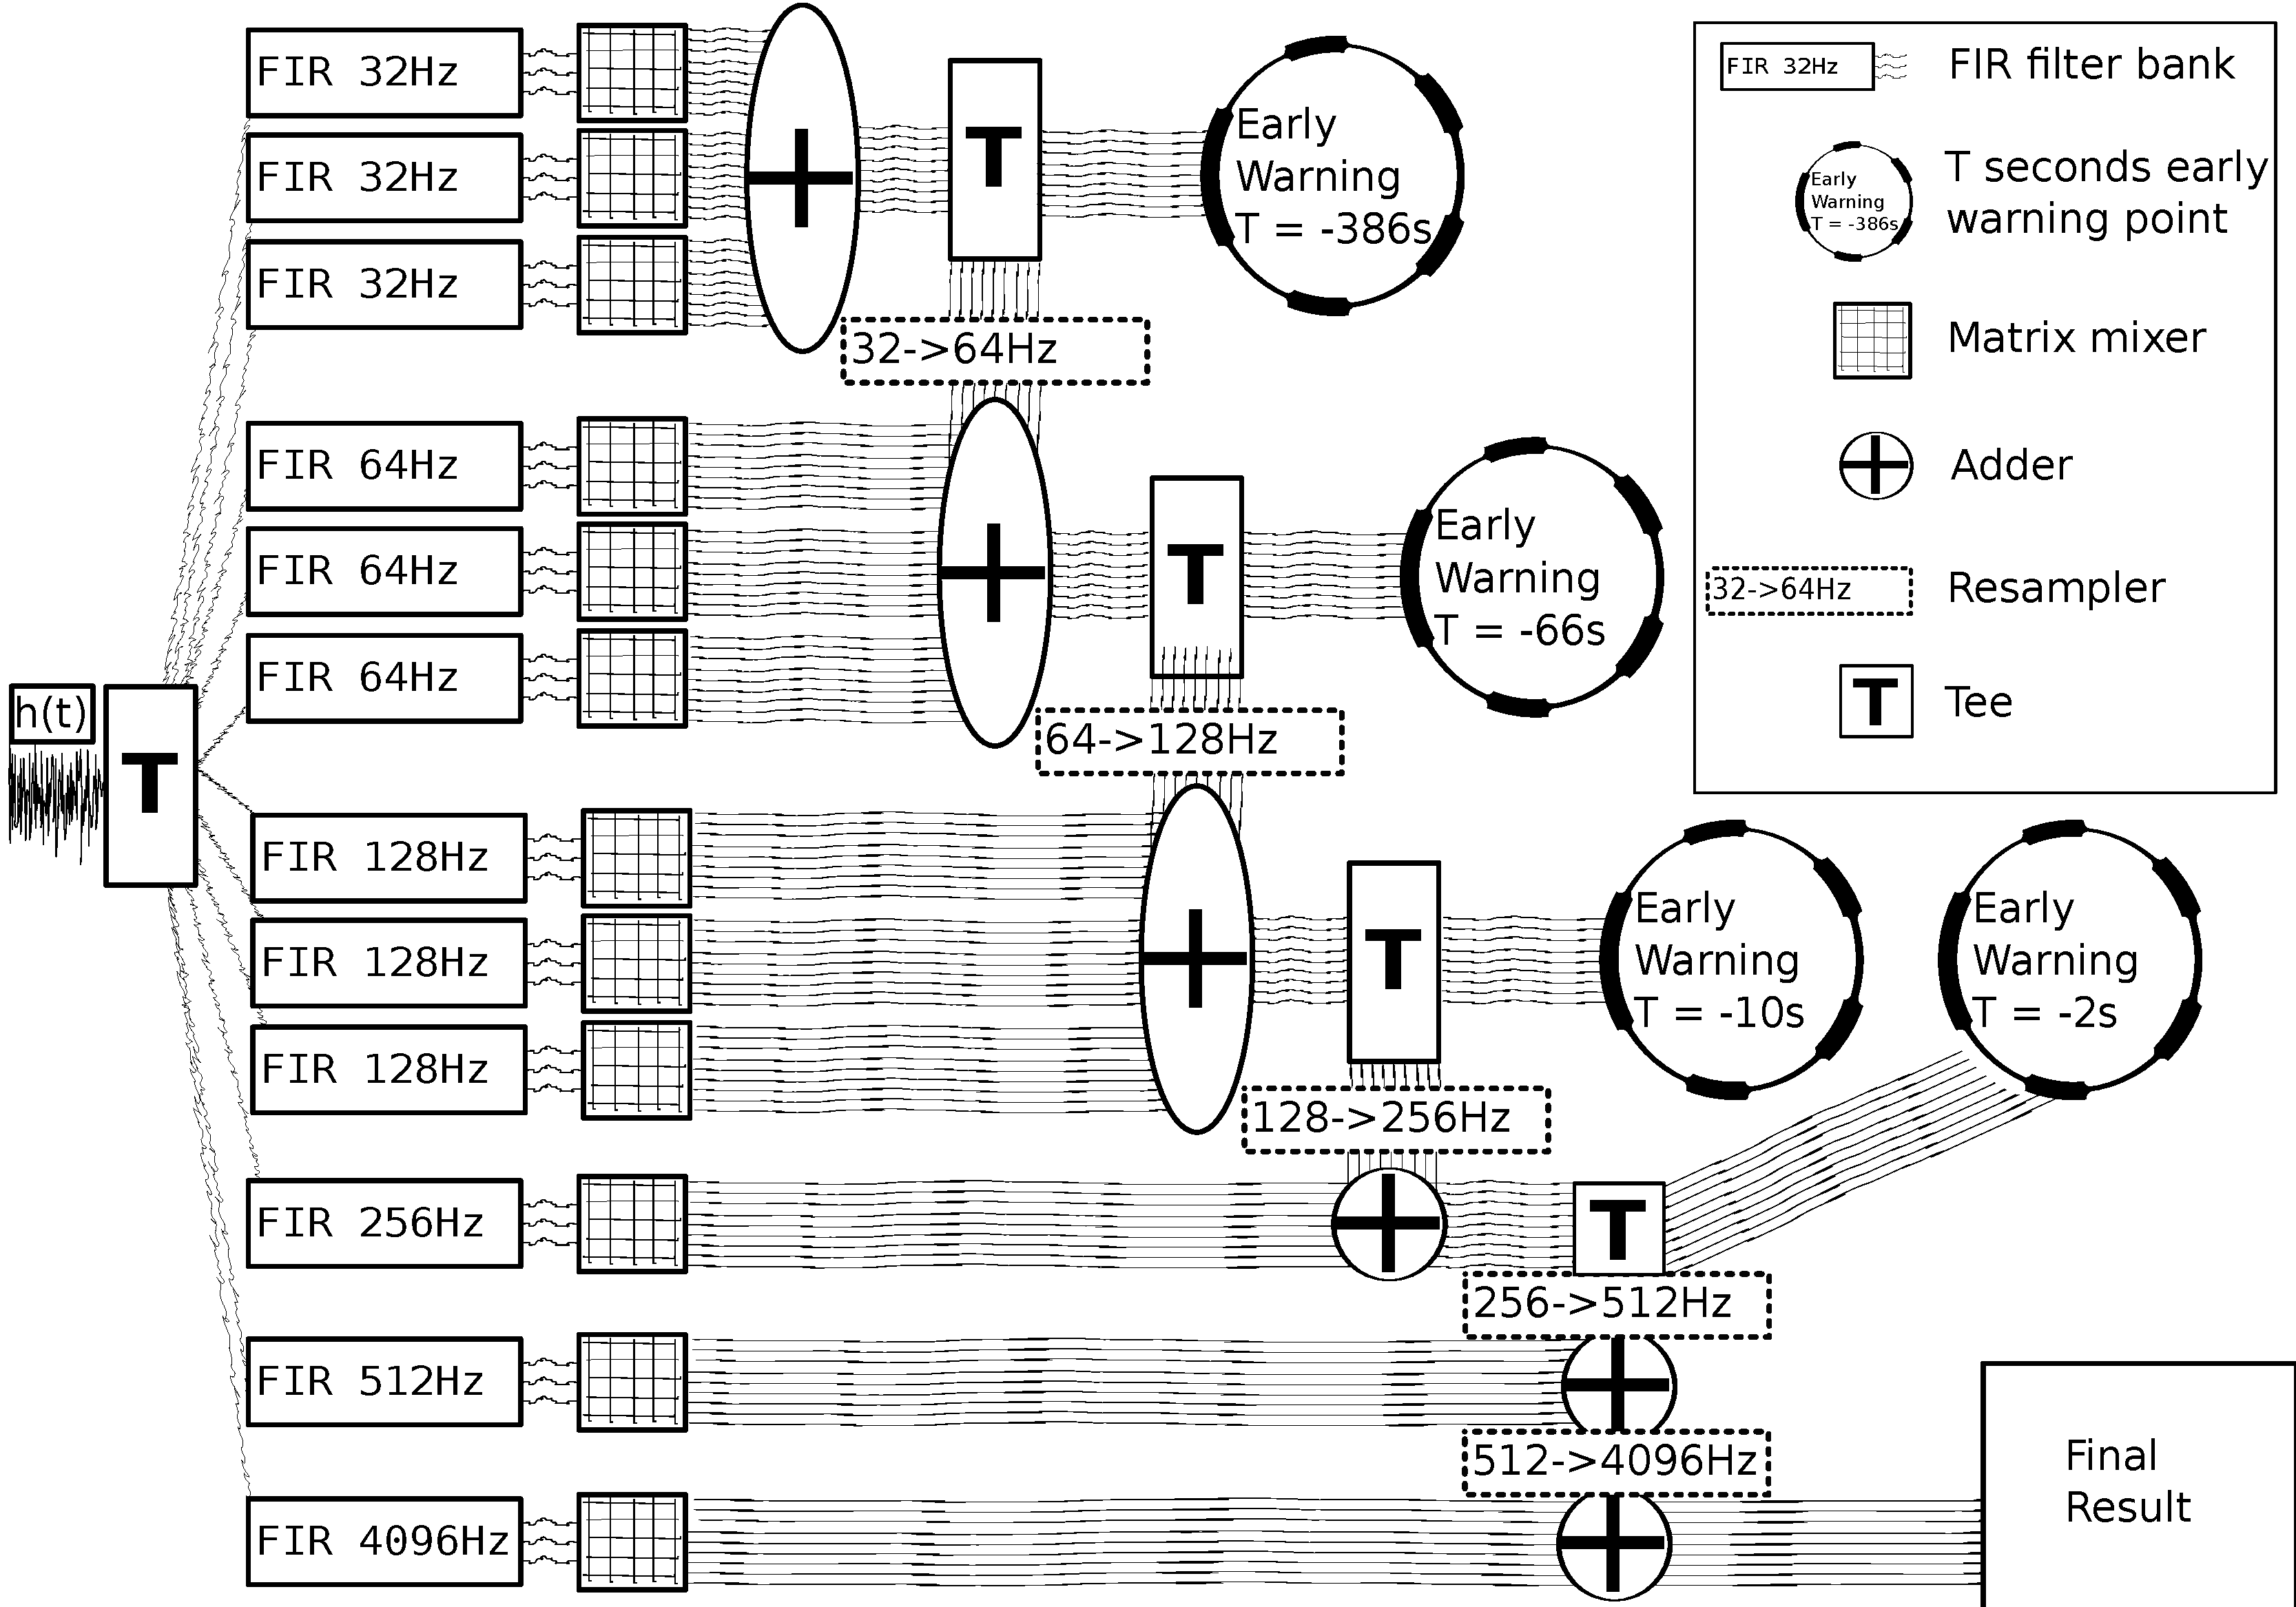
\includegraphics[width=\textwidth]{lloid.pdf}
\caption{Pipeline schematic.}
\end{figure}

\begin{comment}

% Ugly diagram!

\begin{figure*}[h!]
\begin{center}
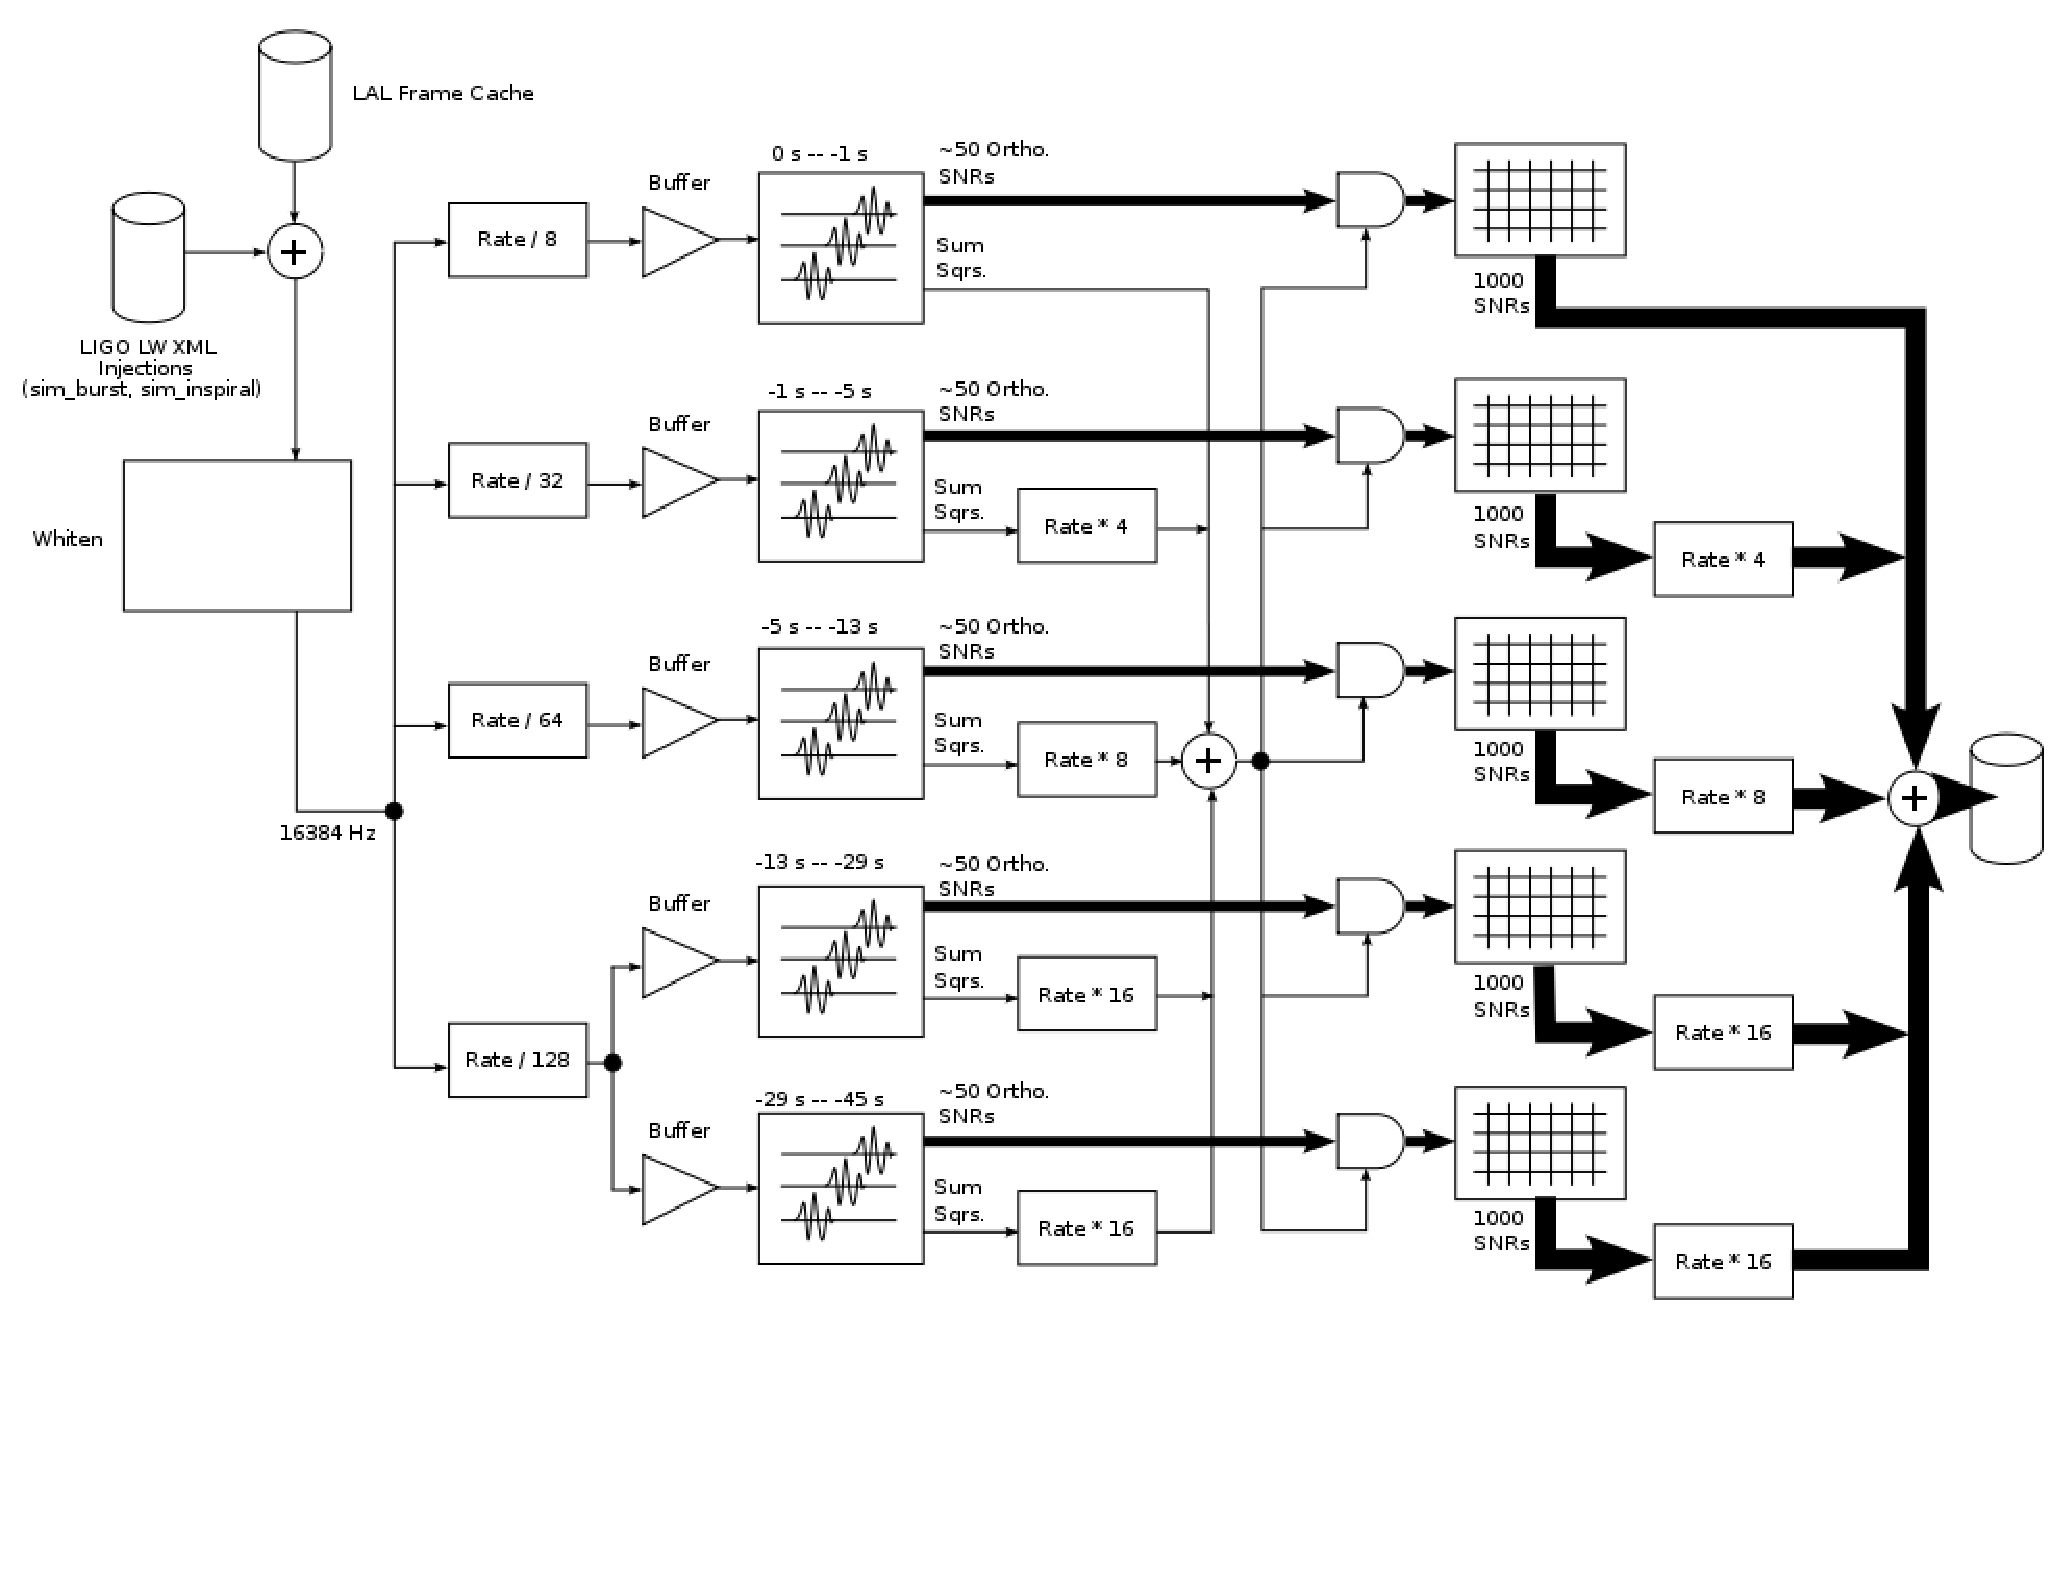
\includegraphics[width=1.0\textwidth]{figures/flow_chart.pdf}
\caption{\label{f:flowchart} 
}
\end{center}
\end{figure*}

\end{comment}
